%\VignetteIndexEntry{Introduction to the USGSwsQWSR package}
%\VignetteEngine{knitr::knitr}
%\VignetteDepends{}
%\VignetteSuggests{xtable}
%\VignettePackage{USGSwsQWSR}

\documentclass[a4paper,11pt]{article}\usepackage[]{graphicx}\usepackage[]{color}
%% maxwidth is the original width if it is less than linewidth
%% otherwise use linewidth (to make sure the graphics do not exceed the margin)
\makeatletter
\def\maxwidth{ %
  \ifdim\Gin@nat@width>\linewidth
    \linewidth
  \else
    \Gin@nat@width
  \fi
}
\makeatother

\definecolor{fgcolor}{rgb}{0.345, 0.345, 0.345}
\newcommand{\hlnum}[1]{\textcolor[rgb]{0.686,0.059,0.569}{#1}}%
\newcommand{\hlstr}[1]{\textcolor[rgb]{0.192,0.494,0.8}{#1}}%
\newcommand{\hlcom}[1]{\textcolor[rgb]{0.678,0.584,0.686}{\textit{#1}}}%
\newcommand{\hlopt}[1]{\textcolor[rgb]{0,0,0}{#1}}%
\newcommand{\hlstd}[1]{\textcolor[rgb]{0.345,0.345,0.345}{#1}}%
\newcommand{\hlkwa}[1]{\textcolor[rgb]{0.161,0.373,0.58}{\textbf{#1}}}%
\newcommand{\hlkwb}[1]{\textcolor[rgb]{0.69,0.353,0.396}{#1}}%
\newcommand{\hlkwc}[1]{\textcolor[rgb]{0.333,0.667,0.333}{#1}}%
\newcommand{\hlkwd}[1]{\textcolor[rgb]{0.737,0.353,0.396}{\textbf{#1}}}%

\usepackage{framed}
\makeatletter
\newenvironment{kframe}{%
 \def\at@end@of@kframe{}%
 \ifinner\ifhmode%
  \def\at@end@of@kframe{\end{minipage}}%
  \begin{minipage}{\columnwidth}%
 \fi\fi%
 \def\FrameCommand##1{\hskip\@totalleftmargin \hskip-\fboxsep
 \colorbox{shadecolor}{##1}\hskip-\fboxsep
     % There is no \\@totalrightmargin, so:
     \hskip-\linewidth \hskip-\@totalleftmargin \hskip\columnwidth}%
 \MakeFramed {\advance\hsize-\width
   \@totalleftmargin\z@ \linewidth\hsize
   \@setminipage}}%
 {\par\unskip\endMakeFramed%
 \at@end@of@kframe}
\makeatother

\definecolor{shadecolor}{rgb}{.97, .97, .97}
\definecolor{messagecolor}{rgb}{0, 0, 0}
\definecolor{warningcolor}{rgb}{1, 0, 1}
\definecolor{errorcolor}{rgb}{1, 0, 0}
\newenvironment{knitrout}{}{} % an empty environment to be redefined in TeX

\usepackage{alltt}

\usepackage{amsmath}
\usepackage{times}
\usepackage{hyperref}
\usepackage[numbers, round]{natbib}
\usepackage[american]{babel}
\usepackage{authblk}
\usepackage{subfig}
\usepackage{placeins}
\usepackage{footnote}
\usepackage{tabularx}
\renewcommand\Affilfont{\itshape\small}

\renewcommand{\topfraction}{0.85}
\renewcommand{\textfraction}{0.1}
\usepackage{graphicx}


\textwidth=6.2in
\textheight=8.5in
\parskip=.3cm
\oddsidemargin=.1in
\evensidemargin=.1in
\headheight=-.3in

%------------------------------------------------------------
% newcommand
%------------------------------------------------------------
\newcommand{\scscst}{\scriptscriptstyle}
\newcommand{\scst}{\scriptstyle}
\newcommand{\Robject}[1]{{\texttt{#1}}}
\newcommand{\Rfunction}[1]{{\texttt{#1}}}
\newcommand{\Rclass}[1]{\textit{#1}}
\newcommand{\Rpackage}[1]{\textit{#1}}
\newcommand{\Rexpression}[1]{\texttt{#1}}
\newcommand{\Rmethod}[1]{{\texttt{#1}}}
\newcommand{\Rfunarg}[1]{{\texttt{#1}}}
\IfFileExists{upquote.sty}{\usepackage{upquote}}{}

\begin{document}






%------------------------------------------------------------
\title{The USGSwsQWSR R package}
%------------------------------------------------------------
\author[1]{Laura De Cicco}
\author[1]{Steve Corsi}
\author[1]{Austin Baldwin}
\affil[1]{United States Geological Survey}






\maketitle
\tableofcontents

%------------------------------------------------------------
\section{Introduction to USGSwsQWSR package}
%------------------------------------------------------------ 
The USGSwsQWSR package was designed to simplify the process of gathering water quality sample data and unit surrogate data, running a stepwise regression using the USGSwsQW censReg function, and analyzing those results. This vignette will first show a general overview workflow  (\ref{sec:workflow}), then a more detailed description of the workflow with working examples (\ref{sec:details}).

%------------------------------------------------------------
\section{General Workflow}
\label{sec:workflow}
%------------------------------------------------------------ 

\begin{knitrout}
\definecolor{shadecolor}{rgb}{0.969, 0.969, 0.969}\color{fgcolor}\begin{kframe}
\begin{alltt}
\hlkwd{library}\hlstd{(}\hlstr{"USGSwsQWSR"}\hlstd{)}

\hlcom{#Sample data included with package:}
\hlstd{DTComplete} \hlkwb{<-} \hlstd{StLouisDT}
\hlstd{UV} \hlkwb{<-} \hlstd{StLouisUV}
\hlstd{QWcodes} \hlkwb{<-} \hlstd{StLouisQWcodes}
\hlstd{siteINFO} \hlkwb{<-} \hlstd{StLouisInfo}

\hlstd{investigateResponse} \hlkwb{<-} \hlstr{"SuspSed"}
\hlstd{transformResponse} \hlkwb{<-} \hlstr{"lognormal"}

\hlstd{DT} \hlkwb{<-} \hlstd{DTComplete[}\hlkwd{c}\hlstd{(investigateResponse,}
                   \hlkwd{getPredictVariables}\hlstd{(}\hlkwd{names}\hlstd{(UV)),}
                   \hlstr{"decYear"}\hlstd{,}\hlstr{"sinDY"}\hlstd{,}\hlstr{"cosDY"}\hlstd{,}\hlstr{"datetime"}\hlstd{)]}
\hlstd{DT} \hlkwb{<-} \hlkwd{na.omit}\hlstd{(DT)}

\hlstd{predictVariables} \hlkwb{<-} \hlkwd{names}\hlstd{(DT)[}\hlopt{-}\hlkwd{which}\hlstd{(}\hlkwd{names}\hlstd{(DT)}
                  \hlopt \hlkwd{c}\hlstd{(investigateResponse,}\hlstr{"datetime"}\hlstd{,}\hlstr{"decYear"}\hlstd{))]}


\hlcom{#Check predictor variables}
\hlkwd{predictVariableScatterPlots}\hlstd{(DT,investigateResponse)}

\hlcom{# Create 'kitchen sink' formula:}
\hlstd{kitchenSink} \hlkwb{<-} \hlkwd{createFullFormula}\hlstd{(DT,investigateResponse)}

\hlcom{#Run stepwise regression with "kitchen sink" as upper bound:}
\hlstd{returnPrelim} \hlkwb{<-} \hlkwd{prelimModelDev}\hlstd{(DT,investigateResponse,kitchenSink,}
                               \hlstr{"BIC"}\hlstd{,} \hlcom{#Other option is "AIC"}
                               \hlstd{transformResponse)}

\hlstd{steps} \hlkwb{<-} \hlstd{returnPrelim}\hlopt{$}\hlstd{steps}
\hlstd{modelResult} \hlkwb{<-} \hlstd{returnPrelim}\hlopt{$}\hlstd{modelStuff}
\hlstd{modelReturn} \hlkwb{<-} \hlstd{returnPrelim}\hlopt{$}\hlstd{DT.mod}

\hlcom{# Analyze steps found:}
\hlkwd{plotSteps}\hlstd{(steps,DT,transformResponse)}
\hlkwd{analyzeSteps}\hlstd{(steps, investigateResponse,siteINFO)}

\hlcom{# Analyze model produced from stepwise regression:}
\hlkwd{resultPlots}\hlstd{(DT,modelReturn,siteINFO)}
\hlkwd{resultResidPlots}\hlstd{(DT,modelReturn,siteINFO)}

\hlcom{# Create prediction plots}
\hlkwd{predictionPlot}\hlstd{(UV,DT,modelReturn,}\hlkwc{siteINFO}\hlstd{=siteINFO)}
\end{alltt}
\end{kframe}
\end{knitrout}



%------------------------------------------------------------
\section{Workflow Details}
\label{sec:details}
%------------------------------------------------------------
In this section, we will step through the basic workflow.

%------------------------------------------------------------
\subsection{Data Retrieval}
%------------------------------------------------------------
Data retrieval is currently supported by web service calls to the National Water Information Service (NWIS). The first step is to get the discrete sample data that the regressions are modeling. In this example, we will look at the St Louis River at Scanlon (USGS site ID 04024000). If we don't know the sample data that is available, we can use the whatQW function to discover that information. 

\begin{knitrout}
\definecolor{shadecolor}{rgb}{0.969, 0.969, 0.969}\color{fgcolor}\begin{kframe}
\begin{alltt}
\hlkwd{library}\hlstd{(USGSwsQWSR)}
\end{alltt}
\end{kframe}
\end{knitrout}






\begin{knitrout}
\definecolor{shadecolor}{rgb}{0.969, 0.969, 0.969}\color{fgcolor}\begin{kframe}
\begin{alltt}
\hlstd{site} \hlkwb{<-} \hlstr{"04024000"}
\hlstd{QWcodes} \hlkwb{<-} \hlkwd{whatQW}\hlstd{(site,} \hlkwc{minCount}\hlstd{=}\hlnum{20}\hlstd{)}
\hlkwd{head}\hlstd{(QWcodes)}
\end{alltt}
\begin{verbatim}
   parameter_cd  startDate    endDate count service
25        00010 1964-10-28 2013-12-30   265      qw
26        00020 1974-10-30 2013-12-30   154      qw
28        00025 1981-10-20 2013-12-30   135      qw
32        00041 2010-10-07 2013-06-11    55      qw
34        00055 2010-10-07 2013-04-27    35      qw
37        00061 1960-07-28 2013-07-17   310      qw
\end{verbatim}
\end{kframe}
\end{knitrout}


Most likely, there will be a known set of parameters that are to be modeled. If the parameter codes for these analytes are known, the data from NWIS can be accessed directly with the function importNWISqw. The following example shows the process, and then lists the column names returned in the QW dataframe.


\begin{knitrout}
\definecolor{shadecolor}{rgb}{0.969, 0.969, 0.969}\color{fgcolor}\begin{kframe}
\begin{alltt}
\hlstd{pCodeQW} \hlkwb{<-} \hlkwd{c}\hlstd{(}\hlstr{"00608"}\hlstd{,}\hlstr{"00613"}\hlstd{,}\hlstr{"00618"}\hlstd{,}\hlstr{"00631"}\hlstd{,}\hlstr{"00665"}\hlstd{,}
             \hlstr{"00671"}\hlstd{,}\hlstr{"00940"}\hlstd{,}\hlstr{"62855"}\hlstd{,}\hlstr{"80154"}\hlstd{)}
\hlstd{startDate} \hlkwb{<-} \hlstr{"2011-03-17"}
\hlstd{endDate} \hlkwb{<-} \hlstr{""}
\hlstd{QW} \hlkwb{<-} \hlkwd{importNWISqw}\hlstd{(site,} \hlkwc{params}\hlstd{=pCodeQW,}
                   \hlkwc{begin.date}\hlstd{=startDate,} \hlkwc{end.date}\hlstd{=endDate)}
\end{alltt}
\end{kframe}
\end{knitrout}





\begin{knitrout}
\definecolor{shadecolor}{rgb}{0.969, 0.969, 0.969}\color{fgcolor}\begin{kframe}
\begin{alltt}
\hlkwd{names}\hlstd{(QW)}
\end{alltt}
\begin{verbatim}
 [1] "site_no"              "sample_dt"           
 [3] "sample_tm"            "tzone_cd"            
 [5] "medium_cd"            "Ammonia.N"           
 [7] "Nitrite.N"            "Nitrate.N"           
 [9] "NO2PlusNO3.N"         "Phosphorus_WW.P"     
[11] "OrthoPhosphate.P"     "Chloride"            
[13] "NitrogenTotal_WW.sum" "SuspSed"             
[15] "datetime"            
\end{verbatim}
\end{kframe}
\end{knitrout}



This brings the data in automatically as a `qw' object. This means that censoring information is embeded within each data point. If any processing needs to be done to the data, it might be easier to import the raw data first, then convert to 'qw' objects with the makeQWObjects function.

\begin{knitrout}
\definecolor{shadecolor}{rgb}{0.969, 0.969, 0.969}\color{fgcolor}\begin{kframe}
\begin{alltt}
\hlstd{QWRaw} \hlkwb{<-} \hlkwd{retrieveNWISqwData}\hlstd{(site,pCodeQW,startDate,}
                            \hlstd{endDate,}\hlkwc{expanded}\hlstd{=}\hlnum{TRUE}\hlstd{)}
\hlstd{QW} \hlkwb{<-} \hlkwd{makeQWObjects}\hlstd{(QWRaw)}
\end{alltt}
\end{kframe}
\end{knitrout}


Next, the unit value data that will be used as surrogates for the analytes should be retrieved. If the parameters are not known, they can be discovered using the getDataAvailability function, filtering just the `uv' (unit value) data:

\begin{knitrout}
\definecolor{shadecolor}{rgb}{0.969, 0.969, 0.969}\color{fgcolor}\begin{kframe}
\begin{alltt}
\hlstd{UVcodes} \hlkwb{<-} \hlkwd{getDataAvailability}\hlstd{(site)}
\hlstd{UVcodes} \hlkwb{<-} \hlstd{UVcodes[UVcodes}\hlopt{$}\hlstd{service} \hlopt{==} \hlstr{"uv"}\hlstd{,]}
\hlkwd{names}\hlstd{(UVcodes)}
\end{alltt}
\begin{verbatim}
 [1] "parameter_cd"       "statCd"            
 [3] "startDate"          "endDate"           
 [5] "count"              "service"           
 [7] "parameter_group_nm" "parameter_nm"      
 [9] "casrn"              "srsname"           
[11] "parameter_units"   
\end{verbatim}
\begin{alltt}
\hlstd{UVcodes}\hlopt{$}\hlstd{parameter_cd}
\end{alltt}
\begin{verbatim}
[1] "00010" "00021" "00060" "00065" "00095" "00300" "00301"
[8] "00400" "63680"
\end{verbatim}
\end{kframe}
\end{knitrout}


Finally, the unit value data can be retrieved with the getMultipleUV function. Because of the potentially large amount of data being returned, the web service call is automatically split into individual parameter codes.

\begin{knitrout}
\definecolor{shadecolor}{rgb}{0.969, 0.969, 0.969}\color{fgcolor}\begin{kframe}
\begin{alltt}
\hlstd{UVpCodes} \hlkwb{<-} \hlkwd{c}\hlstd{(}\hlstr{"00010"}\hlstd{,}\hlstr{"00060"}\hlstd{,}\hlstr{"00095"}\hlstd{,}\hlstr{"00300"}\hlstd{,}\hlstr{"00400"}\hlstd{,}\hlstr{"63680"}\hlstd{)}
\hlstd{UV} \hlkwb{<-} \hlkwd{getMultipleUV}\hlstd{(site, startDate, endDate, UVpCodes)}
\end{alltt}
\end{kframe}
\end{knitrout}





\begin{knitrout}
\definecolor{shadecolor}{rgb}{0.969, 0.969, 0.969}\color{fgcolor}\begin{kframe}
\begin{alltt}
\hlkwd{names}\hlstd{(UV)}
\end{alltt}
\begin{verbatim}
 [1] "agency_cd"   "site_no"     "datetime"    "tz_cd"      
 [5] "Wtemp"       "Wtemp_cd"    "Flow"        "Flow_cd"    
 [9] "SpecCond"    "SpecCond_cd" "DO"          "DO_cd"      
[13] "pH"          "pH_cd"       "Turb"        "Turb_cd"    
\end{verbatim}
\end{kframe}
\end{knitrout}



%------------------------------------------------------------
\subsection{Data Merging}
%------------------------------------------------------------
We now need to merge the sample and continuous data into one dataframe. This is accomplished using the mergeDatasets function.

\begin{knitrout}
\definecolor{shadecolor}{rgb}{0.969, 0.969, 0.969}\color{fgcolor}\begin{kframe}
\begin{alltt}
\hlstd{mergeReturn} \hlkwb{<-} \hlkwd{mergeDatasets}\hlstd{(QW, UV, QWcodes)}
\hlstd{DTComplete} \hlkwb{<-} \hlstd{mergeReturn}\hlopt{$}\hlstd{DTComplete}
\hlstd{QWcodes} \hlkwb{<-} \hlstd{mergeReturn}\hlopt{$}\hlstd{QWcodes}
\end{alltt}
\end{kframe}
\end{knitrout}


The dataframe DTComplete contains a column of each of the discrete samples, and a column of the nearest (temporaly) unit value data. The function mergeDatasets has an argument called `max.diff'. The default is set to `2 hours', meaning that if the sample and continious data timestamps do not match, the merge will take the closest continious data within 2 hours. This value can be changed, see ?mergeNearest for more options.

%------------------------------------------------------------
\subsection{Data Investigation}
%------------------------------------------------------------

%------------------------------------------------------------
\subsubsection{Narrow down investigation}
%------------------------------------------------------------


We now want to narrow our investigation down to one analyte. Let us look at Chloride. First we will want a dataframe DT with just chloride and the unit values. We will call these the `prediciton values' because they will eventually be used to predict chloride.

\begin{knitrout}
\definecolor{shadecolor}{rgb}{0.969, 0.969, 0.969}\color{fgcolor}\begin{kframe}
\begin{alltt}
\hlstd{investigateResponse} \hlkwb{<-} \hlstr{"Chloride"}
\hlstd{predictionVariables} \hlkwb{<-} \hlkwd{getPredictVariables}\hlstd{(}\hlkwd{names}\hlstd{(UV))}

\hlstd{DT} \hlkwb{<-} \hlstd{DTComplete[}\hlkwd{c}\hlstd{(investigateResponse,}
                   \hlstd{predictionVariables,}
                   \hlstr{"decYear"}\hlstd{,}\hlstr{"sinDY"}\hlstd{,}\hlstr{"cosDY"}\hlstd{,}\hlstr{"datetime"}\hlstd{)]}

\hlkwd{names}\hlstd{(DT)}
\end{alltt}
\begin{verbatim}
 [1] "Chloride" "Wtemp"    "Flow"     "SpecCond" "DO"      
 [6] "pH"       "Turb"     "decYear"  "sinDY"    "cosDY"   
[11] "datetime"
\end{verbatim}
\end{kframe}
\end{knitrout}


For the regression, there can be no NA values in any of the columns. There are many ways in R to deal with this requirement. The easiest way to do it is remove any row that has any NA. This can be done as follows:

\begin{knitrout}
\definecolor{shadecolor}{rgb}{0.969, 0.969, 0.969}\color{fgcolor}\begin{kframe}
\begin{alltt}
\hlstd{DT} \hlkwb{<-} \hlkwd{na.omit}\hlstd{(DT)}
\end{alltt}
\end{kframe}
\end{knitrout}


There may be other situations where you want to remove a column that contains the majority of the missing data.

%------------------------------------------------------------
\subsubsection{Plot variables}
%------------------------------------------------------------
There are a few tools included in this package to explore the data before performing the regression.

\begin{knitrout}
\definecolor{shadecolor}{rgb}{0.969, 0.969, 0.969}\color{fgcolor}\begin{kframe}
\begin{alltt}
\hlkwd{plotQQTransforms}\hlstd{(DT,investigateResponse)}
\end{alltt}
\end{kframe}\begin{figure}[]

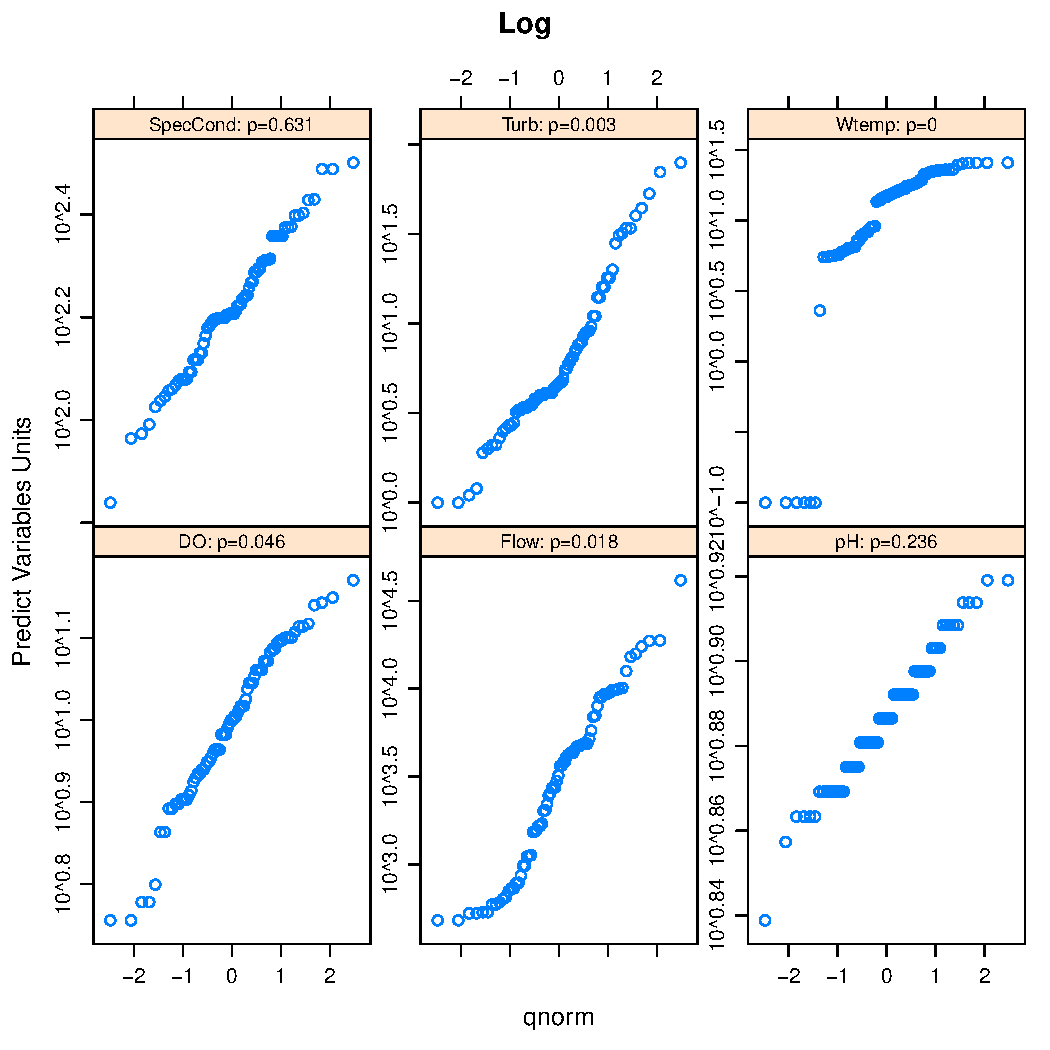
\includegraphics[width=\maxwidth]{figure/plotQQTransforms1} \caption[plotQQTransforms]{plotQQTransforms\label{fig:plotQQTransforms1}}
\end{figure}

\begin{figure}[]

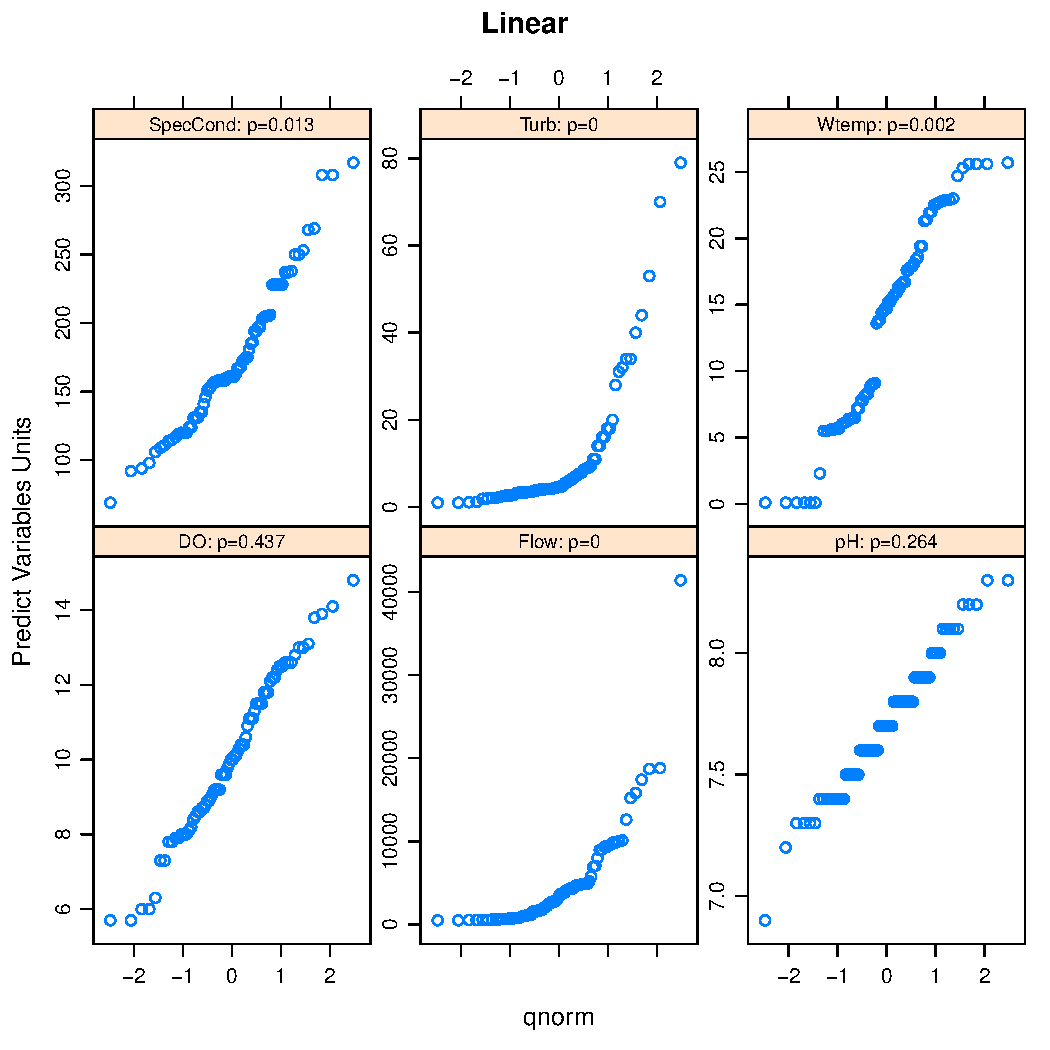
\includegraphics[width=\maxwidth]{figure/plotQQTransforms2} \caption[plotQQTransforms]{plotQQTransforms\label{fig:plotQQTransforms2}}
\end{figure}


\end{knitrout}



\begin{knitrout}
\definecolor{shadecolor}{rgb}{0.969, 0.969, 0.969}\color{fgcolor}\begin{kframe}
\begin{alltt}
\hlkwd{predictVariableScatterPlots}\hlstd{(DT,investigateResponse)}
\end{alltt}
\end{kframe}\begin{figure}[]

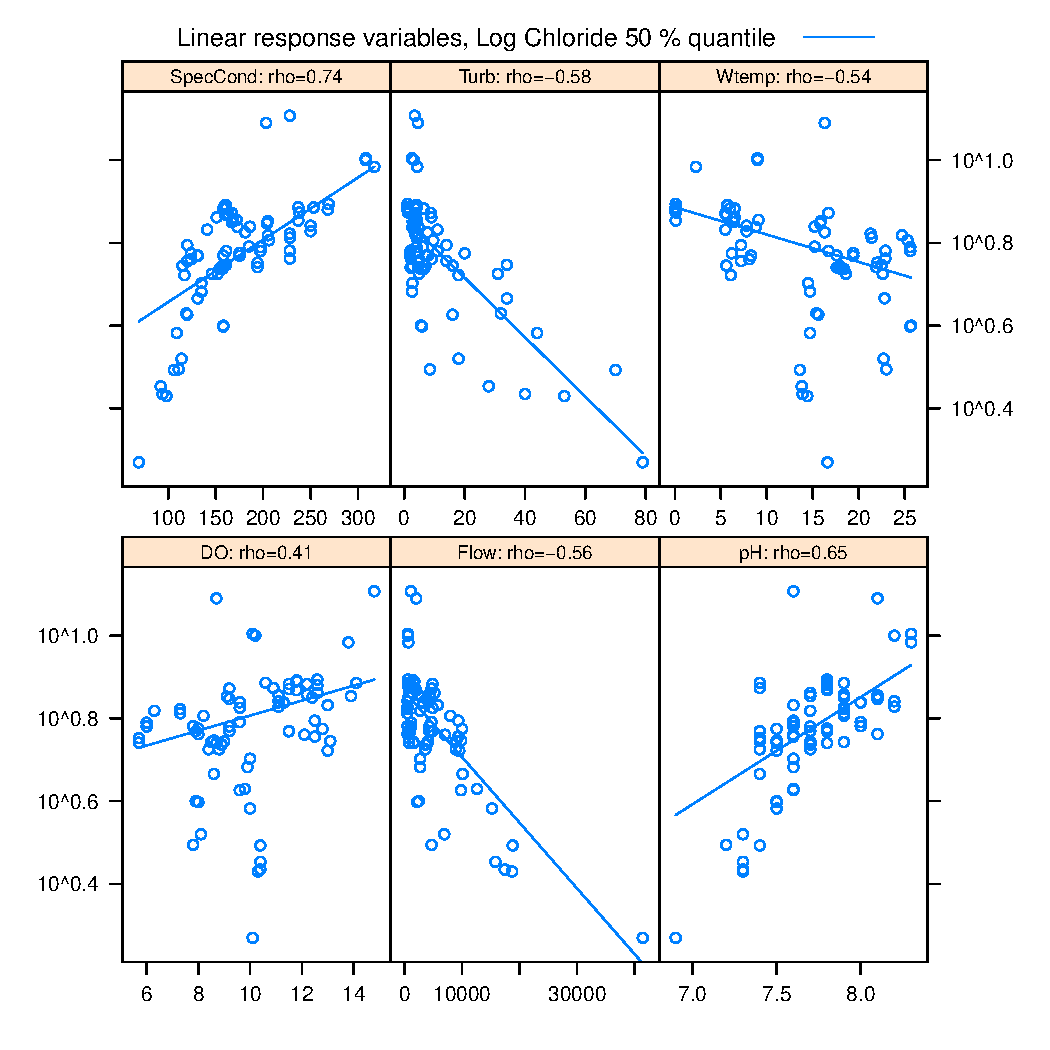
\includegraphics[width=\maxwidth]{figure/predictVariableScatterPlots1} \caption[predictVariableScatterPlots]{predictVariableScatterPlots\label{fig:predictVariableScatterPlots1}}
\end{figure}

\begin{figure}[]

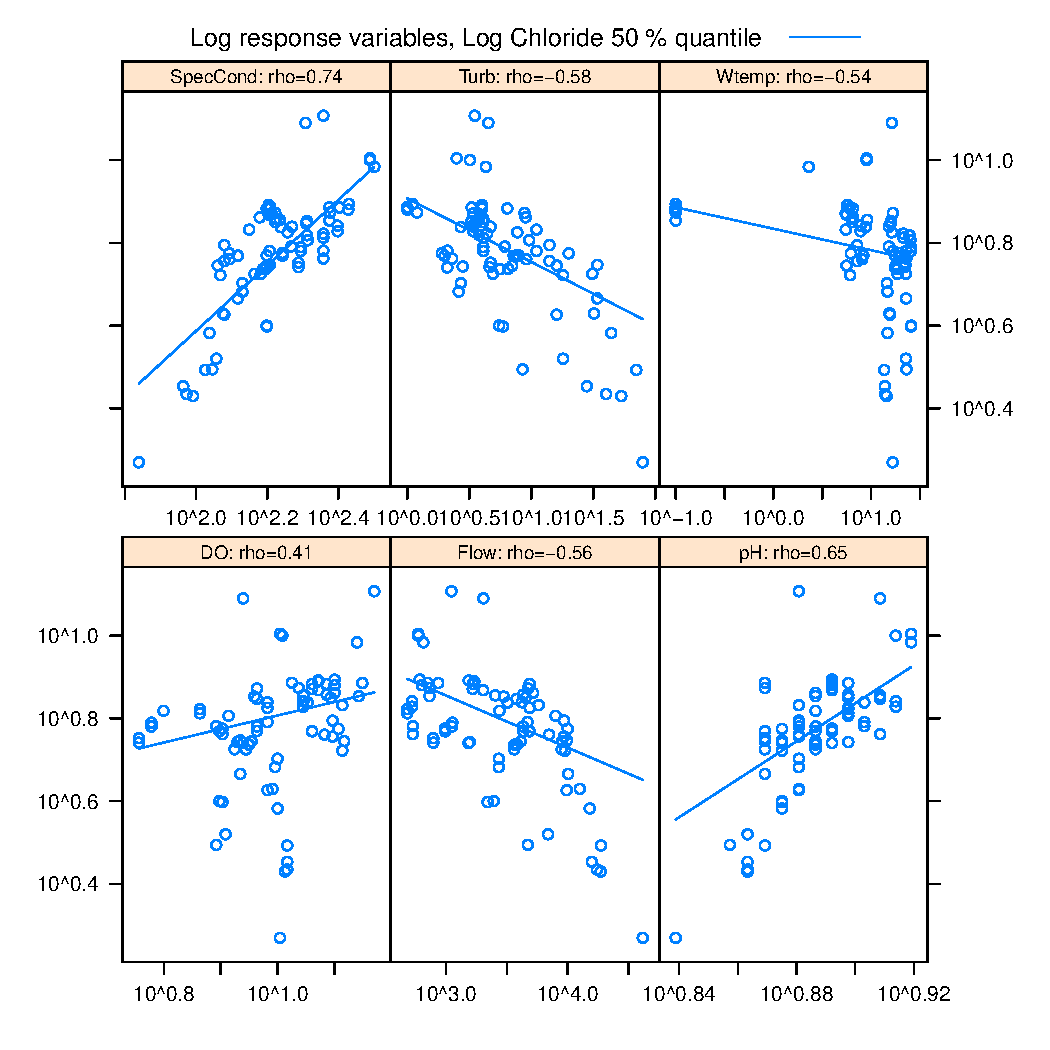
\includegraphics[width=\maxwidth]{figure/predictVariableScatterPlots2} \caption[predictVariableScatterPlots]{predictVariableScatterPlots\label{fig:predictVariableScatterPlots2}}
\end{figure}


\end{knitrout}


\FloatBarrier
%------------------------------------------------------------
\subsection{Stepwise Regression}
%------------------------------------------------------------

%------------------------------------------------------------
\subsection{Model Analysis}
%------------------------------------------------------------

\clearpage
\appendix

%------------------------------------------------------------ 
\section{Getting Started in R}
\label{sec:appendix1}
%------------------------------------------------------------ 
This section describes the options for downloading and installing the dataRetrieval package.

%------------------------------------------------------------
\subsection{New to R?}
%------------------------------------------------------------ 
If you are new to R, you will need to first install the latest version of R, which can be found here: \url{http://www.r-project.org/}.

There are many options for running and editing R code, one nice environment to learn R is RStudio. RStudio can be downloaded here: \url{http://rstudio.org/}. Once R and RStudio are installed, the dataRetrieval package needs to be installed as described in the next section.

At any time, you can get information about any function in R by typing a question mark before the functions name.  This will open a file (in RStudio, in the Help window) that describes the function, the required arguments, and provides working examples.

\begin{knitrout}
\definecolor{shadecolor}{rgb}{0.969, 0.969, 0.969}\color{fgcolor}\begin{kframe}
\begin{alltt}
\hlkwd{library}\hlstd{(USGSwsQWSR)}
\hlopt{?}\hlstd{plotSteps}
\end{alltt}
\end{kframe}
\end{knitrout}


To see the raw code for a particular code, type the name of the function:
\begin{knitrout}
\definecolor{shadecolor}{rgb}{0.969, 0.969, 0.969}\color{fgcolor}\begin{kframe}
\begin{alltt}
\hlstd{plotSteps}
\end{alltt}
\end{kframe}
\end{knitrout}


%------------------------------------------------------------
\subsection{R User: Installing QWSR}
%------------------------------------------------------------ 
Before installing USGSwsQWSR, the dependent packages must be first be installed:

\begin{knitrout}
\definecolor{shadecolor}{rgb}{0.969, 0.969, 0.969}\color{fgcolor}\begin{kframe}
\begin{alltt}
\hlkwd{install.packages}\hlstd{(}\hlkwd{c}\hlstd{(}\hlstr{"XML"}\hlstd{,} \hlstr{"lubridate"}\hlstd{,} \hlstr{"akima"}\hlstd{,} \hlstr{"KernSmooth"}\hlstd{,}
                   \hlstr{"leaps"}\hlstd{,} \hlstr{"car"}\hlstd{,} \hlstr{"mvtnorm"}\hlstd{,} \hlstr{"digest"}\hlstd{,}
                   \hlstr{"relimp"}\hlstd{,} \hlstr{"BSDA"}\hlstd{,} \hlstr{"RODBC"}\hlstd{,}\hlstr{"memoise"}\hlstd{,}
                   \hlstr{"boot"}\hlstd{,}\hlstr{"survival"}\hlstd{,}\hlstr{"splines"}\hlstd{,}\hlstr{"RColorBrewer"}\hlstd{,}
                   \hlstr{"lattice"}\hlstd{,}\hlstr{"MASS"}\hlstd{),}
                 \hlkwc{dependencies}\hlstd{=}\hlnum{TRUE}\hlstd{)}
\hlkwd{install.packages}\hlstd{(}\hlkwd{c}\hlstd{(}\hlstr{"USGSwsBase"}\hlstd{,}\hlstr{"USGSwsData"}\hlstd{,}\hlstr{"dataRetrieval"}\hlstd{,}
                   \hlstr{"USGSwsGraphs"}\hlstd{,}\hlstr{"USGSwsStats"}\hlstd{,}
                   \hlstr{"USGSwsQW"}\hlstd{,}\hlstr{"USGSwsQWSR"}\hlstd{),} \hlkwc{repos}\hlstd{=}\hlstr{"http://usgs-r.github.com"}\hlstd{)}
\end{alltt}
\end{kframe}
\end{knitrout}



After installing the package, you need to open the library each time you re-start R.  This is done with the simple command:
\begin{knitrout}
\definecolor{shadecolor}{rgb}{0.969, 0.969, 0.969}\color{fgcolor}\begin{kframe}
\begin{alltt}
\hlkwd{library}\hlstd{(USGSwsQWSR)}
\end{alltt}
\end{kframe}
\end{knitrout}





\end{document}
